To measure the memorability of individual objects from our dataset, we created an alternate version of the Visual Memory Game following the basic design in \cite{isola11}, with the exception of a few key differences. We administered the game and collected data through Amazon Mechanical Turk. In our game, participants first viewed a sequence of images one at a time, with a $1.5$ second gap in between image presentations. Subjects were asked to remember the contents and objects inside those images as much as they could. To ensure that subjects would not just only look at the salient or center objects, subjects had unlimited time to freely view the images. Once they were done viewing an image, they could press any key to advance to the next image. Following the initial image sequence, participants then viewed a sequence of objects, their task then being to indicate through a key press which of those objects was present in one of the previously shown images. Each object was displayed for $1.5$ second, with a $1.5$ second gap in between the object sequences. Pairs of corresponding image and object sequences were broken up into $10$ blocks. Each block consisted of $80$ total stimuli ($35$ images and $45$ objects), and lasted approximately $3$ minutes. At the end of each block, the subject could take a short break. Overall, the experiment took approximately took $30$ minutes to complete.


\begin{figure}[t]
\centering
\subfigure{\centering 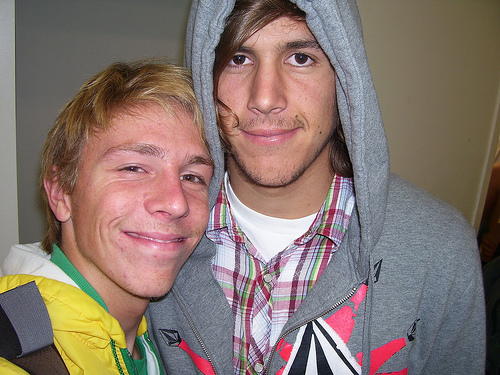
\includegraphics[width=0.1\textwidth]{figures/method/18.jpg}}
\subfigure{\centering 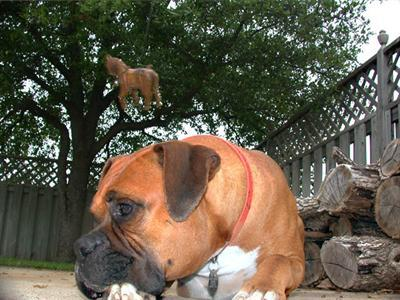
\includegraphics[width=0.1\textwidth]{figures/method/1288.jpg}}
\subfigure{\centering 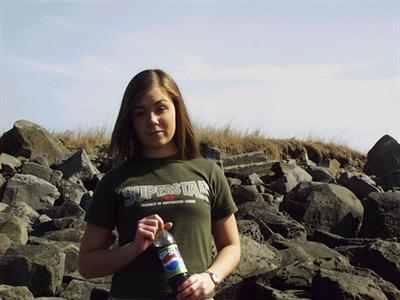
\includegraphics[width=0.1\textwidth]{figures/method/1409.jpg}}
\subfigure{\centering 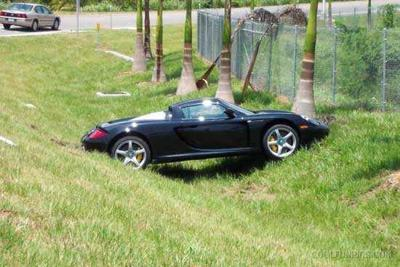
\includegraphics[width=0.1\textwidth]{figures/method/filler5.jpg}}\\
\subfigure{\centering 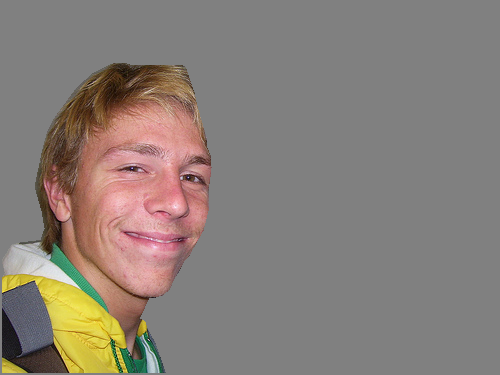
\includegraphics[width=0.1\textwidth]{figures/method/18_4.png}}
\subfigure{\centering 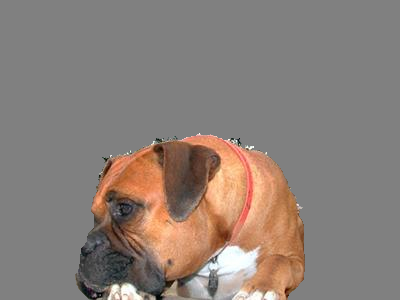
\includegraphics[width=0.1\textwidth]{figures/method/1288.png}}
\subfigure{\centering 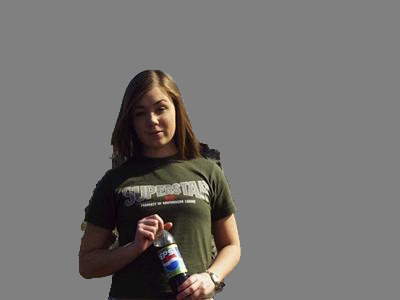
\includegraphics[width=0.1\textwidth]{figures/method/1409.png}}
\subfigure{\centering 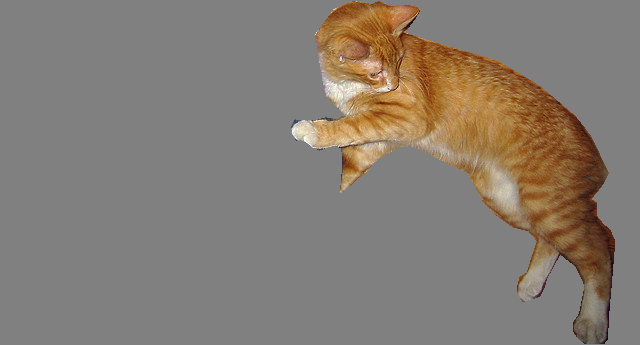
\includegraphics[width=0.1\textwidth]{figures/method/15297.png}}
\vspace{-5mm}\caption{\footnotesize\textbf{Example stimuli from the memory game.} Example filler, familiar, and control images and objects. }\label{fig:exampleStimuli}
\end{figure}

Unknown to the subjects, inside each block, each sequence of images was pseudo-random and consisted of $3$ 'target' images taken from the Pascal-S dataset whose objects the participants were to later identify. The remaining images in the sequence consisted of $16$ 'filler' images and $16$ 'familiar' images. The 'filler' images were randomly selected from the DUT-OMRON dataset \cite{dutomron13} and the 'familiar' images were randomly sampled from the MSRA dataset proposed in \cite{msra11}. Similarly, the object sequence was also pseudo-random and consisted of $3$ 'target' objects ($1$ object taken randomly from each previously shown target image). The remaining objects in the sequence consisted of $10$ 'control' objects, $16$ 'filler' objects, and $16$ 'familiar' objects. The 'filler' objects were taken randomly from the $80$ different object categories in the Microsoft COCO dataset \cite{coco14} and the 'familiar' objects were the objects taken from the previously displayed 'familiar' images in the image sequence. The filler images and objects helped provide spacing between the target images and target objects, whereas the familiar images and objects allowed us to check if the subjects were paying attention to the task \cite{brady08}, \cite{isola11}. While the fillers and familiars (both the images and objects) were taken from datasets resembling real world scenes and objects, the 'control' objects were artificial stimuli randomly sampled from the dataset proposed in \cite{brady08} and helped serve as an additional control to test the attentiveness of the subjects. Repeats on targets i.e. the target images and target objects were spaced $70-79$ stimuli apart, and repeats occurred on the familiars with a spacing of $1-79$ stimuli (i.e. distance between familiar images and their objects). The images and objects appeared only once, and each subject was tested on only one object from each target image. Objects were centered within their parent frame and non-object pixels were set to grey. Participants were required to complete the entire task, which included $10$ blocks (overall time approximately $30$ minutes), and could not participate in the experiment a second time. After collecting the data, we assigned a 'memorability score' to each target object in our dataset, defined as the percentage of correct detections by subjects. In all our analysis, we removed all subjects whose accuracy on the control objects was below $75\%$ and below $50\%$ on familiar images/objects. A total of \textcolor{red}{$2000$} workers from Mechanical Turk ($> 95\%$ approval rate in Amazon’s system) performed the game and on average each object was scored by $20$ subjects. 